% !TEX TS-program = xelatex
% !TEX TS-options = -synctex=1

\documentclass[12pt]{article}

\usepackage{amssymb,amsmath, amsfonts,eurosym,geometry,ulem,graphicx,caption,subcaption,color,setspace,sectsty,comment,footmisc,natbib,pdflscape,array,hyperref, mathtools,bbm, longtable}


% \usepackage[nomarkers,notablist,nofiglist]{endfloat}
\usepackage{threeparttable}
\usepackage{adjustbox}
\usepackage{booktabs}
\usepackage{tikz}
% \renewcommand{\efloatseparator}{\medskip}
\usepackage{fancyhdr}
\usepackage[ruled, vlined]{algorithm2e}
\usepackage{float}
\usepackage{appendix}
\normalem

% \onehalfspacing
% \newtheorem{theorem}{Theorem}
% \newtheorem{corollary}[theorem]{Corollary}
% \newtheorem{prop}{Proposition}
% \newenvironment{proof}[1][Proof]{\noindent\textbf{#1.}}{\ \rule{0.5em}{0.5em}}

% \newtheorem{hyp}{Hypothesis}
% \newtheorem{subhyp}{Hypothesis}[hyp]
% \renewcommand{\thesubhyp}{\thehyp\alph{subhyp}}
\usepackage{amsthm}
\onehalfspacing
\newtheorem{theorem}{Theorem}
\newtheorem{corollary}[theorem]{Corollary}
\newtheorem{prop}{Proposition}
\newtheorem{hyp}{Hypothesis}
\newtheorem{subhyp}{Hypothesis}[hyp]
\renewcommand{\thesubhyp}{\thehyp\alph{subhyp}}

\newcommand{\red}[1]{{\color{red} #1}}
\newcommand{\blue}[1]{{\color{blue} #1}}

\newcolumntype{L}[1]{>{\raggedright\let\newline\\arraybackslash\hspace{0pt}}m{#1}}
\newcolumntype{C}[1]{>{\centering\let\newline\\arraybackslash\hspace{0pt}}m{#1}}
\newcolumntype{R}[1]{>{\raggedleft\let\newline\\arraybackslash\hspace{0pt}}m{#1}}

\geometry{left=1.0in,right=1.0in,top=1.0in,bottom=1.0in}

\begin{document}
\begin{titlepage}
\title{Title}
\author{Kohei Kawaguchi}
\date{\today}
\maketitle
\begin{abstract}
\noindent

\bigskip
\end{abstract}
\setcounter{page}{0}
\thispagestyle{empty}
\end{titlepage}
\pagebreak \newpage

Cite \cite{aguirregabiriaDynamicsMarkupsInventories1999}.

\begin{figure}[H]
    \centering
    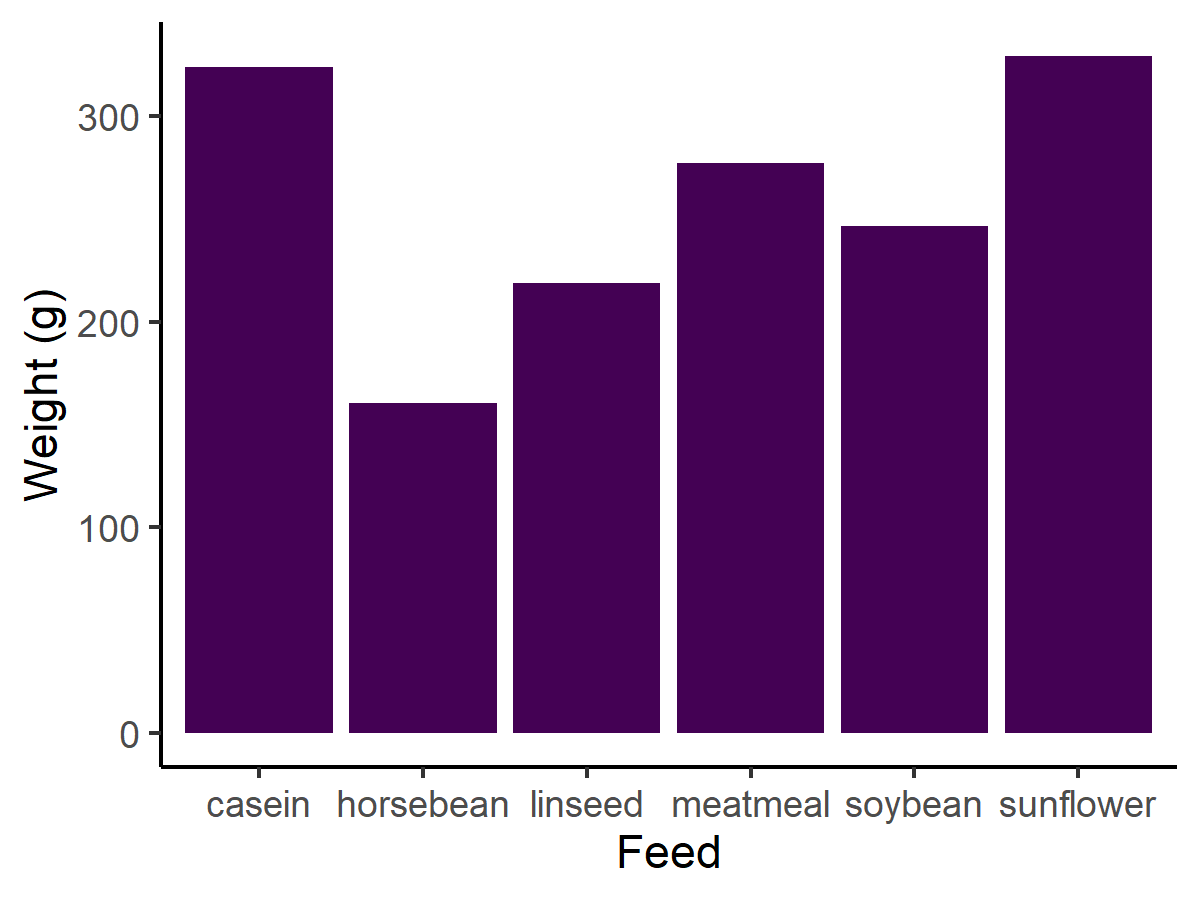
\includegraphics[width=0.8\textwidth]{figuretable/tutorial_figure_bar_ggplot2.png}
    \caption{Figure}
\end{figure}

\singlespacing
\setlength\bibsep{0pt}
\bibliographystyle{aer.bst}
\bibliography{library.bib}

\end{document}